\documentclass[a4paper, 11pt]{article}
\usepackage{comment}
\usepackage{lipsum} 
\usepackage{fullpage} %cambiar margen
\usepackage[a4paper, total={7in, 10in}]{geometry}

\usepackage{amssymb,amsthm} 
\usepackage{amsmath}
\newtheorem{theorem}{Theorem}
\newtheorem{corollary}{Corollary}
\usepackage{graphicx}
\usepackage{tikz}
\usetikzlibrary{arrows}
\usepackage{verbatim}
%\usepackage[numbered]{mcode}
\usepackage{float}
\usepackage{tikz}
\usetikzlibrary{shapes,arrows}
\usetikzlibrary{arrows,calc,positioning}
\usepackage{mathpazo} %tipo de letra 
\usepackage[utf8]{inputenc} %codificación
\usepackage[T1]{fontenc} %digitación de tildes y ñ
\usepackage[spanish]{babel} %paquete de soporte español

\tikzset{
	block/.style = {draw, rectangle,
		minimum height=1cm,
		minimum width=1.5cm},
	input/.style = {coordinate,node distance=1cm},
	output/.style = {coordinate,node distance=4cm},
	arrow/.style={draw, -latex,node distance=2cm},
	pinstyle/.style = {pin edge={latex-, black,node distance=2cm}},
	sum/.style = {draw, circle, node distance=1cm},
}
\usepackage{xcolor}
\usepackage{mdframed}
\usepackage[shortlabels]{enumitem}
\usepackage{indentfirst}
\usepackage{hyperref}

\usepackage{listings}
\lstset{literate=
  {á}{{\'a}}1
  {é}{{\'e}}1
  {í}{{\'i}}1
  {ó}{{\'o}}1
  {ú}{{\'u}}1
  {Á}{{\'A}}1
  {É}{{\'E}}1
  {Í}{{\'I}}1
  {Ó}{{\'O}}1
  {Ú}{{\'U}}1
  {ñ}{{\~n}}1
  {ü}{{\"u}}1
  {Ü}{{\"U}}1
}

\lstdefinestyle{customc}{
  belowcaptionskip=1\baselineskip,
  breaklines=true,
  frame=L,
  xleftmargin=\parindent,
  language=Python,
  showstringspaces=false,
  basicstyle=\footnotesize\ttfamily,
  keywordstyle=\bfseries\color{green!40!black},
  commentstyle=\itshape\color{purple!40!black},
  identifierstyle=\color{blue},
  stringstyle=\color{orange},
}

\lstdefinestyle{customasm}{
  belowcaptionskip=1\baselineskip,
  frame=L,
  xleftmargin=\parindent,
  language=[x86masm]Assembler,
  basicstyle=\footnotesize\ttfamily,
  commentstyle=\itshape\color{purple!40!black},
}

\lstset{escapechar=@,style=customc}



\renewcommand{\thesubsection}{\thesection.\alph{subsection}}

\newenvironment{problem}[2][Ejercicio]
{ \begin{mdframed}[backgroundcolor= red!50] \textbf{#1 #2} \\}
	{  \end{mdframed}}

% Define solution environment
\newenvironment{solution}
{\textcolor{blue}{\textbf{\textit{Solución:\\\noindent}}}}


\renewcommand{\qed}{\quad\qedsymbol}

% \\	
\begin{document}
	\noindent
	%%%%%%%%%%%%%%%%%%%%%%%%%%%%%%%%%%%%
	
	\begin{minipage}[b][1.2cm][t]{0.8\textwidth}
		\large\textbf{César Isaí García Cornejo} \hfill \textbf{Tarea 2}  \\
		cesar.cornejo@cimat.mx \hfill \\
		\normalsize Computo Científico \hfill Semestre 3\\
	\end{minipage}
	
	\hspace{14.4cm}
	\begin{minipage}[b][0.03cm][t]{0.12\linewidth}
		
		\vspace{-2.2cm}
		%%%La Ruta dependera de donde este alojado el main y la imagen
		
\includegraphics[scale=0.3]{Figures/EscudoCimat.png}
	\end{minipage}
	
	\noindent\rule{7in}{2.8pt}
	
	%%%%%%%%%%%%%%%%%%%%%
	%%%%%%%%%%%%%%%%%%%%%%%%%%%%%%%%%%%%%%%%%%%%%%%%%%%%%%%%%%%%%%%%%%%%%%%%%%%%%%%%%%%%%%%%%%%%%%%%%%%%%%%%%%%%%%%%%%%
	% Problem 1
	%%%%%%%%%%%%%%%%%%%%%%%%%%%%%%%%%%%%%%%%%%%%%%%%%%%%%%%%%%%%%%%%%%%%%%%%%%%%%%%%%%%%%%%%%%%%%%%%%%%%%%%%%%%%%%%%%%%%%%%%%%%%%%%%%%%%%%%%
	\setlength{\parskip}{\medskipamount}
	\setlength{\parindent}{0pt}
%/////////// Ejercicio 1 /////////////////
\begin{problem}{1}
    Implementar el algoritmo de Gram-Schmidt modificado 8.1 del Trefethen (p.58) para generar la descomoposición QR.
\end{problem}

\begin{solution}
Usando la tería de los proyectores ortogonales es que se encuetra un algoritmo mas \textit{estable} para hacer Gram-Schmidt. Es decir se tiene un algoritmo para hacer factorización QR reducida. 

El algoritmo implementado es tal que se ingresa una matriz $A$ de dimensiones $m \times n$ y regresa una factoriazión de la forma
\begin{align*}
    A = \hat{Q} \hat{R}
\end{align*}
donde $\hat{Q}$ y $\hat{R}$ son matrices de dimensión $m \times n$ y $n \times n $, respectivamente. Además la matriz $\hat{R}$ es una matriz triangular superior. 

El código implementado en Python se basa en lo siguiente
\begin{lstlisting}
    for i in range(n):
        
        R[i,i] = np.sqrt(np.dot(V[:,i],V[:,i]))
        Q[:,i] = V[:,i] / R[i,i]

        for j in range(i+1,n):

            R[i,j] = np.dot(Q[:,i], V[:,j]) 
            V[:,j] = V[:,j] - R[i,j] * Q[:,i]
\end{lstlisting}

donde el vector $V$ es una copia de la matriz de entrada 
$A$.

Por dar un ejemplo consideremos que se desea factorizar la matriz
\begin{align*}
    \begin{bmatrix}
        1 & 2 & 2\\
        2 & 0 & 2\\
        0 & 1 & 2\\
    \end{bmatrix}
\end{align*}
tras aplicar la función GramSchmidt a la matriz A resulta en 
\begin{align*}
    A = QR = 
    \begin{bmatrix}
        0.4472136 & 0.78072006 & -0.43643578\\
        0.89442719 & -0.39036003 & 0.21821789\\
        0. & 0.48795004 & 0.87287156\\
    \end{bmatrix}
    \begin{bmatrix}
        2.23606798 & 0.89442719 & 2.68328157\\
        0. & 2.04939015 & 1.75662013\\
        0. & 0. & 1.30930734\\
    \end{bmatrix}
\end{align*}
que tras hacer la multiplicación matricial de la derecha se comprueba que es en efecto una factorización de A.

\end{solution}


%/////////// Ejercicio 2 /////////////////
\begin{problem}{2}
    Implementar el algoritmo que calcula el estimador de mínimos cuadrados de una regresión usando la descomposición QR.
\end{problem}

\begin{solution}

Consideremos el problema de mínimos cuadrados donde nos interesa encontrar $\hat{x }$ que minimice la relación en $b = Ax$ bajo la norma en $L^2$
\begin{align}
    \hat{x} = argmin_{x}||b - Ax||
    \label{2.01}
\end{align}

Sabemos que la solución a (\ref{2.01}) es
\begin{align*}
    y = A x 
\end{align*}
donde $Pb = y$ y $P = QQ*$ es el proyector ortogonal. Luego el estimador de minimos cuadrados satisface
\begin{align}
    QQ*b &= QR\hat{x },\nonumber \\
    Q*b &= R\hat{x}
    \label{2.02}
\end{align}
por lo que resta resolver el sistema de ecuaciones, y como $R$ es una matriz triangular superior, entonces por medio de \textit{backward subsection} se obtiene el estimador de mínimos cuadrados.

Por dar un ejemplo, consideremos la matriz de diseño
\begin{align*}
    A = 
    \begin{bmatrix}
        1 & 2 & 0\\
        1 & 7 & 2\\
        1 & 7 & 9\\
        1 & 4 & 5\\
      \end{bmatrix}
\end{align*}
y vector respuesta
\begin{align*}
    b = 
    \begin{bmatrix}
        1\\
        2\\
        3\\
        1\\
      \end{bmatrix}
\end{align*}
por tanto usando la función construida para hacer descomposión QR y los comandos 
\begin{lstlisting}

A = np.array([[1,2,0],[1,7,2],[1,7,9],[1,4,5]])

b = np.array([[1],[2],[3],[1]])

Q, R = GramSchmidtModified(A)

b_hat = Q.T @ b

x = backward(R,bhat)

\end{lstlisting}

Tenemos las siguientes matrices
\begin{align*}
    QR = 
    \begin{bmatrix}
        0.5 & -0.70710678 & -0.21320072\\
        0.5 & 0.47140452 & -0.71066905\\
        0.5 & 0.47140452 & 0.56853524\\
        0.5 & -0.23570226 & 0.35533453\\
      \end{bmatrix}
      \begin{bmatrix}
        2. & 10. & 8.\\
        0. & 4.24264069 & 4.00693843\\
        0. & 0. & 5.47215172\\
      \end{bmatrix}
\end{align*}

Además se obtiene el resultado, que es el estimador de mínimos cuadrados 
\begin{align}
    \hat{x } = \begin{bmatrix}
        0.13961039\\ 0.25974026 \\ 0.07792208\\
      \end{bmatrix}
      \label{2.03}
\end{align}

por tanto el modelo de regresión lineal es
\begin{align}
    b_i = x_1 + a_{i1} x_2 + a_{i3}  x_3
\end{align}
donde los $x_i$ están dados en (\ref{2.03}).

\end{solution}




\begin{problem}{3}
    Generar $\mathbf{Y }$ compuesto de $y_i = sen (x_i ) +\epsilon_i $ donde $\epsilon_i \sim N(0,\sigma)$ con $\sigma = 0.11$ para $x_i = \frac{4\pi i }{n }$ para $i = 1,\cdots, n$. 

    Hacer un ajuste de mínimos cuadrados a \textbf{Y}, con descomposición QR, ajustando un polinomio de grado $p-1$.
    \begin{enumerate}
        \item Considerar los 12 casos: p = 3,4,6, 100 y n = 100, 1000, 10000.
        \item Graficar el ajuste en cada caso.
        \item Medir el tiempo de ejecución de su algoritmo, comparar con la descomposición QR de scipy y graficar los resultados.
    \end{enumerate}
\end{problem}

\begin{solution}
    Se construyo una función que recrea el experimento mencionado en el enunciado superior. Es decir, tomamos una regresión polinomial de grado $p-1$. El regresor x es una particion del intervalo $[0,4\pi]$ y la variable respuesta es una tranformación del regresor más el error que distribuye normal estandar. Se generaron los $n$ puntos. Se uso regresión con factorización QR tal como se detallo en el ejercicio previo. Luego se graficaron los resultados de la regresión que se muestran a continuación.

    \begin{figure}[H]
        \centering
        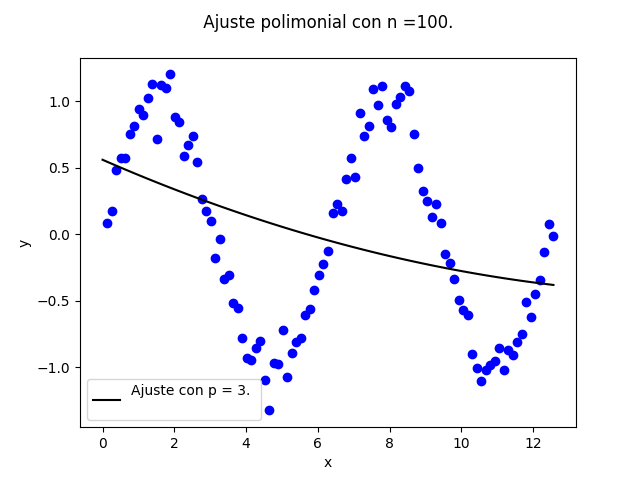
\includegraphics[width = 14cm]{Figures/fig1.png}
        \label{3.01}
    \end{figure}

    \begin{figure}[H]
        \centering
        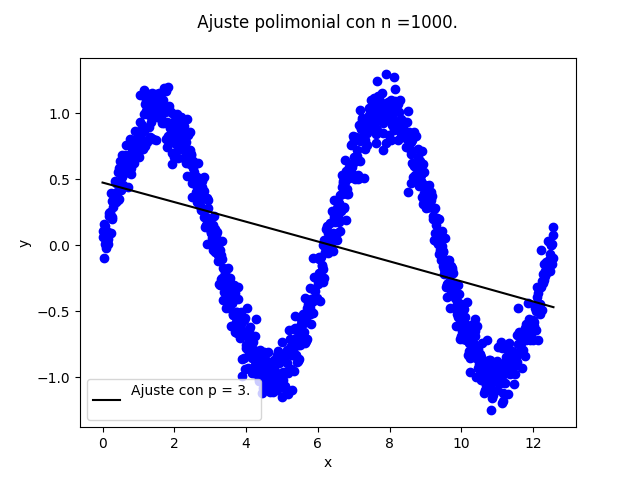
\includegraphics[width = 14cm]{Figures/fig2.png}
        \label{3.02}
    \end{figure}

    \begin{figure}[H]
        \centering
        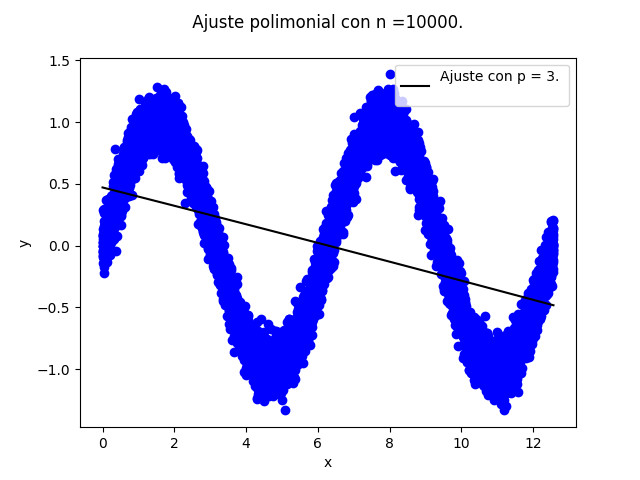
\includegraphics[width = 14cm]{Figures/fig3.png}
        \label{3.03}
    \end{figure}

    \begin{figure}[H]
        \centering
        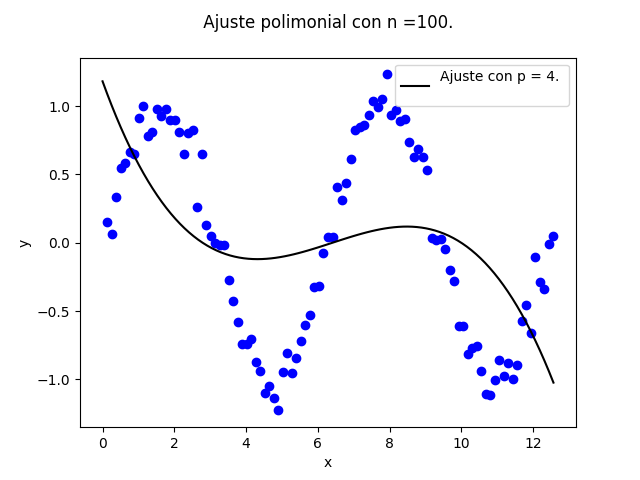
\includegraphics[width = 14cm]{Figures/fig4.png}
        \label{3.04}
    \end{figure}

    \begin{figure}[H]
        \centering
        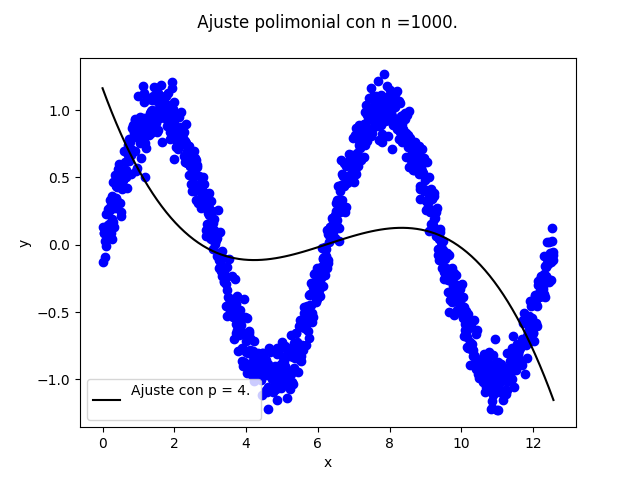
\includegraphics[width = 14cm]{Figures/fig5.png}
        \label{3.05}
    \end{figure}

    \begin{figure}[H]
        \centering
        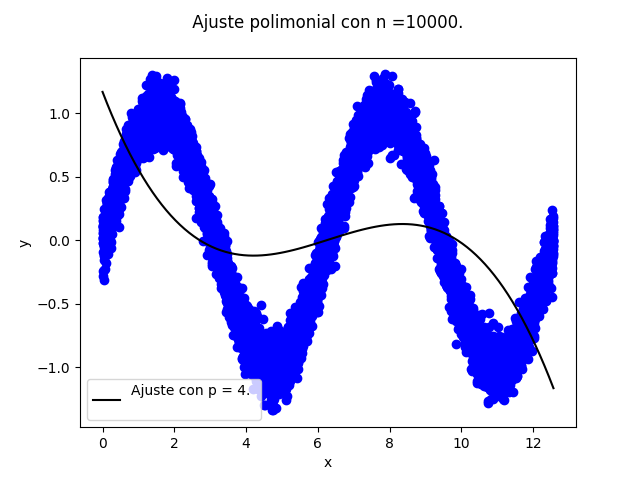
\includegraphics[width = 14cm]{Figures/fig6.png}
        \label{3.06}
    \end{figure}

    \begin{figure}[H]
        \centering
        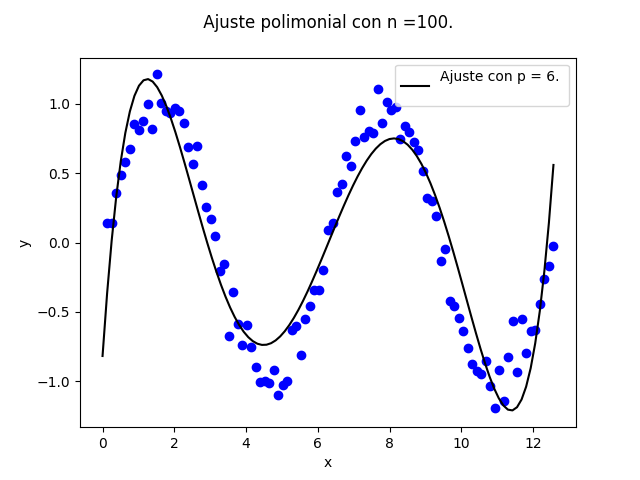
\includegraphics[width = 14cm]{Figures/fig7.png}
        \label{3.07}
    \end{figure}

    \begin{figure}[H]
        \centering
        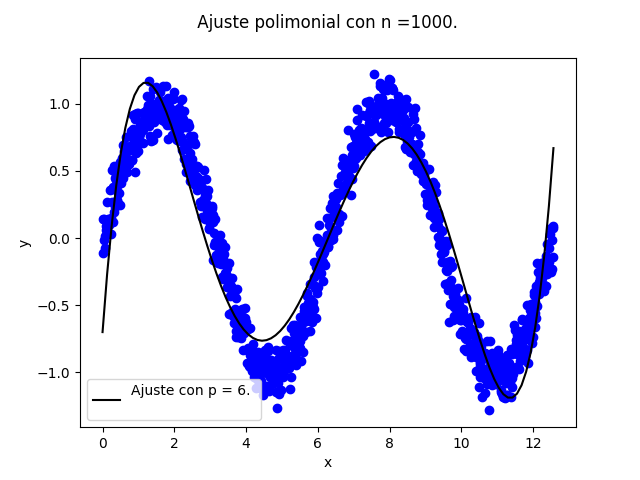
\includegraphics[width = 14cm]{Figures/fig8.png}
        \label{3.08}
    \end{figure}

    \begin{figure}[H]
        \centering
        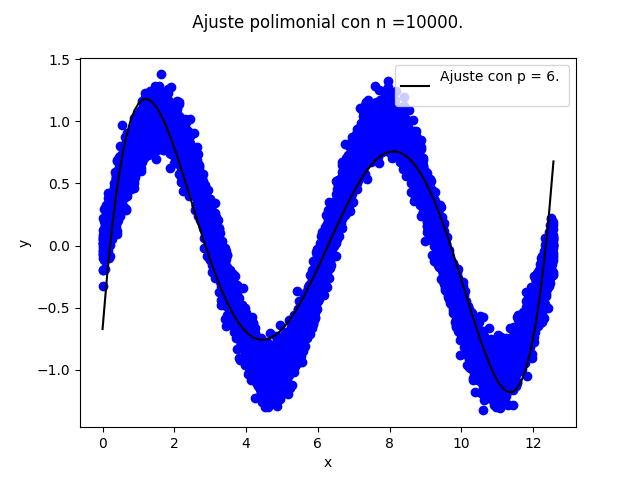
\includegraphics[width = 14cm]{Figures/fig9.png}
        \label{3.09}
    \end{figure}

    \begin{figure}[H]
        \centering
        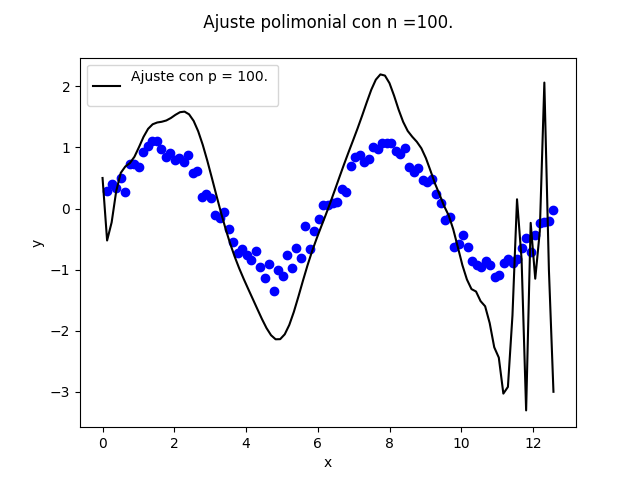
\includegraphics[width = 14cm]{Figures/fig10.png}
        \label{3.10}
    \end{figure}

    \begin{figure}[H]
        \centering
        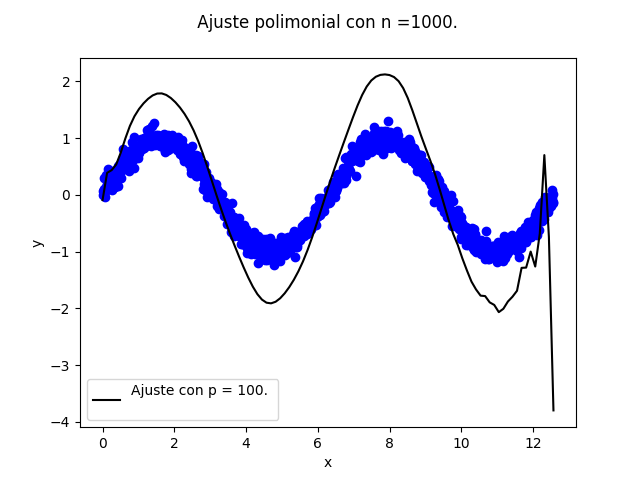
\includegraphics[width = 14cm]{Figures/fig11.png}
        \label{3.11}
    \end{figure}

    \begin{figure}[H]
        \centering
        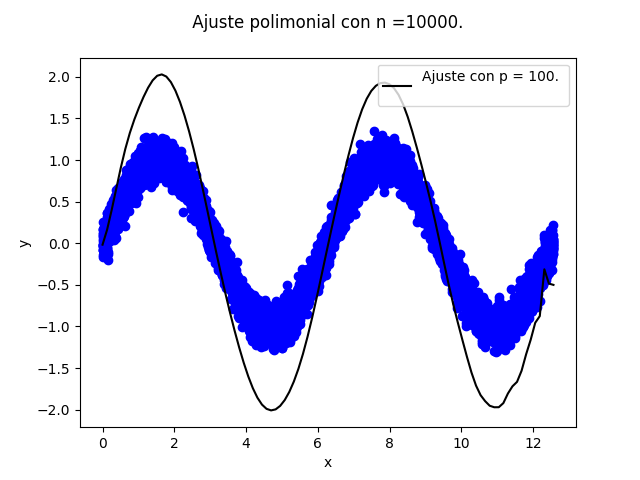
\includegraphics[width = 14cm]{Figures/fig12.png}
        \label{3.12}
    \end{figure}

Observemos que las gráficas son bastante intuitivas a excepción de la gráfica con $n = p = 100$ pues el ajuste debería pasar por cada valor en la muestra ya que la matriz de diseño esta completamente determinada. Sin embargo este es un problema de la graficación, pues el dominio se partio con un \textit{linspace} con solo 100 subdivisiones. Se puede ver en la siguiente figura que si aumentamos dicho número para mayor presición vemos que el ajuste pasa por los datos, aunque por defecto del ajuste lineal los extremos tienden a crecer desproporcionadamente.

\begin{figure}[H]
    \centering
    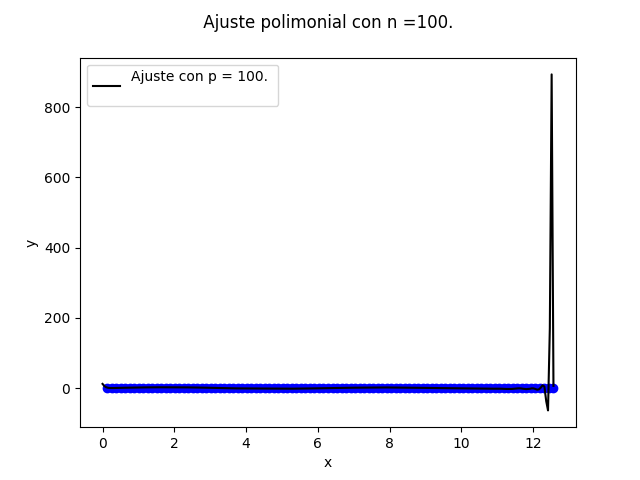
\includegraphics[width = 14cm]{Figures/patologico.png}
    \label{3.13}
\end{figure}

\end{solution}

% //////////////// Ejercicio 4 //////////
\begin{problem}{4}
    Hacer $p = 0.1n$, o sea, diez veces más observaciones que coeficientes en la regresión, ?` Cuál es la $n$ máxima que puede generar su computadora?
\end{problem}

\begin{solution}
    
    
    Vemos que el valor de $n$ máximo es 50000. En un estado natural el comportamiento de la memoria esta cerca del 40 por cieto de uso, como lo vemos en la siguiente figura
    \begin{figure}[H]
        \centering
        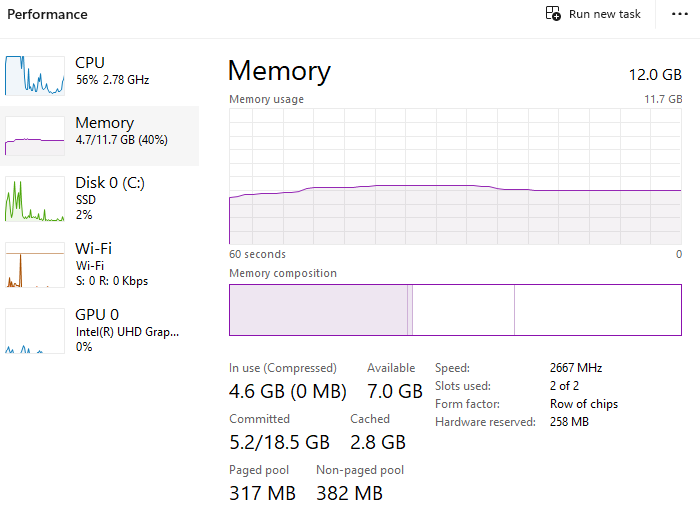
\includegraphics[width = 14cm]{Figures/memory2.png}
        \label{4.1}
    \end{figure}
    
    En el caso de $n$ cercano a 50000 la memoria se mantine estable pero el proceso no termina. Vemos los requerimientos en la siguiente figura.
    
    \begin{figure}[H]
        \centering
        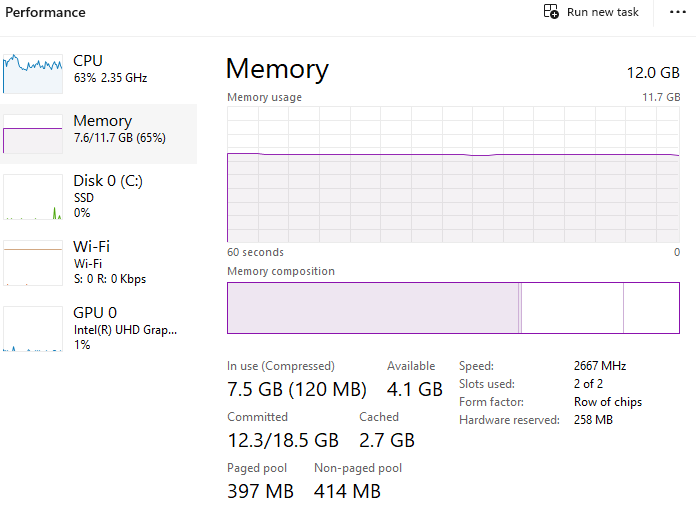
\includegraphics[width = 14cm]{Figures/memoria4.png}
        \label{4.2}
    \end{figure}
    
    Sin embargo en casos mayores se observa una creciente consumo de memoria y capacidad de CPU por lo que el proceso termina por fracturarse.
    
    \begin{figure}[H]
        \centering
        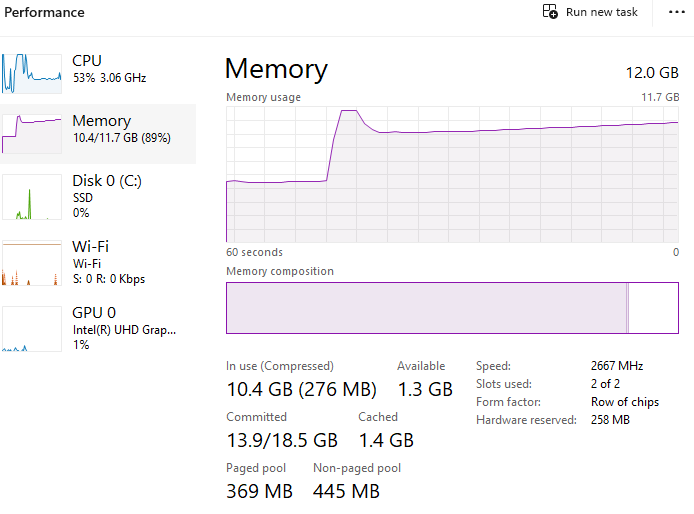
\includegraphics[width = 14cm]{Figures/memoria5.png}
        \label{4.3}
    \end{figure}
    
\end{solution}
    
    \end{document}